\documentclass[preprint,5p,authoryear]{elsarticle}

\usepackage{amsmath}
\usepackage{amsfonts}
\usepackage{graphicx}
\usepackage[small]{caption}
\usepackage[subrefformat=parens]{subcaption}
\usepackage{booktabs}
\usepackage{multirow}
\usepackage{rotating}
\usepackage{url}
\usepackage[table]{xcolor}
\usepackage{hyperref}

\journal{NeuroImage}

\bibliographystyle{elsarticle-harv}

\begin{document}

\begin{frontmatter}

\title{Identifying virtual-world stimulus information from fMRI data}

\author[UT]{Andrew Floren\corref{cor}}
\ead{afloren@utexas.edu}

\author[UT]{Bruce Naylor}

\author[UT]{David Ress}

\address[UT]{The University of Texas at Austin, Austin, TX 78712 USA}

\cortext[cor]{Corresponding author.}

\begin{abstract}
abstract
\end{abstract}

\begin{keyword}
keyword1 \sep keyword2
\end{keyword}

\end{frontmatter}

\section{Introduction}
When conducting research using functional magnetic resonance imaging (fMRI) and the blood oxygen level dependent (BOLD) signal to analyze how the brain responds to stimuli, static experimental paradigms have been the dominant choice.
Such work has generally attempted to focus on a single variable of interest and create stimuli that isolate that aspect.
While this has proven to be a successful approach, it does not mimic the dynamically changing environment in which the primate brain has evolved.
More natural and dynamic stimuli will evoke a more complex network of brain responses.
These complex responses can make interpretation difficult, but it is important to test whether currently accepted neural correlates remain valid in more natural settings because the context in which a stimuli is presented could affect how it is processed.
Researchers have begun using dynamic stimuli in the form of prerecorded movies and, to a lesser extent, virtual reality (VR) environments.

Although difficult, interpreting complex stimuli is not intractable; \cite{Hasson2004} showed that subjects can exhibit relatively homogeneous functional activation when viewing natural and complex stimuli (the movie \emph{The Good, the Bad and the Ugly}).
More complex stimuli require more complex analysis methods.
In \cite{Spiers2007}, the authors review a number of experiments that use either movies or VR and discussed the wide variety of methods used to interrogate these dynamic stimuli: general linear models (GLM), statistical parametric mapping (SPM), independent component analysis (ICA), reverse correlation, and multi-voxel pattern analysis (MVPA) being among the most popular.
These analysis methods can generally be split into stimulus-driven methods -- such as GLM and SPM -- which measure the statistical significance of a hypothesis, and data-driven methods -- such as ICA and MVPA -- which look for patterns in the fMRI signal.
Stimulus-driven analyses provide more easily interpretable results but become less and less tractable as the complexity of the stimulus increases.
Data-driven analyses, on the other hand, can cope with more complex stimuli but are difficult to interpret in terms of understanding how the brain works.
Ideally, data-driven analyses should be used to uncover hidden patterns in complex stimuli which in turn are used to help formulate hypotheses and design stimuli to be tested by stimulus-driven analyses.
\emph{we could move these last couple of sentences to discussion but I was hoping to assuage GLM and SPM diehards.}

MVPA is a data-driven analysis method that has been used in a wide variety of applications \citep{Haxby2001,Mitchell2003,Haynes2006} and has seen an increase in popularity lately.
However, MVPA has been used as somewhat of a blanket term for the application of any machine learning algorithm to fMRI data.
When applying these algorithms, the stimulus is typically organized into multiple categories or classifications (e.g. houses, faces, tools etc.).
(add more info on general machine learning).
This is in contrast to utlizing a General Linear Model (GLM), which treats each voxel independently as a time-series of responses over an extended period of time.
Discuss timing issues.
Discuss sensitivity, search light in particular.

Although prerecorded movies have been used more frequently for dynamic stimuli, VR stimuli have a number of inherent advantages.
Virtual worlds have two advantages over videos of the real world: 1) the stimulus designer has complete control over the stimuli 2) the subject can interact with the virtual world by making a sequence of decisions while in the scanner.
First and foremost, very precise control can be exercised over VR environments.
Second, manipulating variables in the presentation of a VR environment is much less time consuming than recording multiple videos.
Third, the environment can be automatically coded.
That is, the presence or absence of faces, apparent motion, etc. can all be extracted for each frame directly from the stimulus without requiring manual viewing and labeling of each frame.
Finaly, VR stimuli allow for real-time interaction and feedback.
However, VR does have some disadvantages.
Recording a movie is generally much easier than programming a VR environment.
Movies are also generally more realistic looking than VR environments.
The results presented in \cite{Han2005} indicate that there is some divergence in the way the brain processes real, that is recorded, and virtual visual worlds. 
However, cartoons were used to represent virtual visual worlds in this study, and it is likely that as the realism of VR environments increases this divergance in processing will decrease.

Although underutilized, VR stimuli have been used for sometime, including positron emission tomography (PET) experiments.
In \cite{Maguire1998}, the authors use PET and a VR stimuli to study brain regions associated with navigation and internal spacial representations. 
In \cite{Calhoun2002}, the authors use fMRI and a VR stimuli to study brain regions associated with driving.
In \cite{King2005}, the authors use fMRI and a VR stimuli to study brain regions associated with episodic memory.
In \cite{King2006}, the authors use fMRI and a VR stimuli to study brain regions associated with identifying appropriate and inappropriate behavior.
In \cite{Mathiak2006}, the authors use fMRI and a VR stimuli to study brain regions associated with violent behavior.
In \cite{Spiers2007a}, the authors use fMRI and a VR stimuli to study brain regions associated with driving behavior.
All of the studies discusses so far used stimulus-driven analysis methods, that is, some form of GLM or SPM anlysis.
In \cite{Hassabis2009}, the authors used MVPA to analyze their experiment which used fMRI and a VR stimulus to study brain regions associated with internal representations of space in the hippocampus.

More recently, the use of VR stimuli has waned.
However, there are still a number of groups utilizing dynamic stimuli in the form of movies.
In \cite{Chadwick2010}, the authors use fMRI and a movie stimulus to decode episodic memories in the hippocampus.
MVPA was used to analyze this experiment.
In \cite{Nishimoto2011}, the authors use fMRI and a movie stimulus to decode the visual experience of a subject using a generative functional activation model.
Interestingly, this experiment was analyzed using a stimulus-driven method unlike most recent decoding experiments which employ MVPA.
The results were positive, but the complex modelling required illustrates the difficulties of such an approach.

The application of MVPA analysis to VR stimuli can create some very exciting experimental possibilities.
However, the difficulty of designing and building VR environments along with complexities of applying and interpreting MVPA analysis have limited the utilization of this combination.
We hope that by rigorously exploring the methodologies involved in applying MVPA to VR stimuli we can increase their utilization.
\emph{we could potentially move the last few sentences to discussion but I want to get the reader into the mindset of methodology before introducing our experiment}
We test the feasibility of extracting complex information from fMRI data while subjects view natural and dynamic stimuli.
Our experiment was structured to identify those parts of the brain that are related to the perception and apparent number of human characters in a scene.
Unlike previous experiments that examined the neural correlates of object counting or number evaluation \citep{countingstuff}, we used a passive-viewing stimulus paradigm.
To analyze the fMRI data from our more complex stimuli, we employed MVPA.
More specifically, we tested two different machine learning algorithms: the support vector machine (SVM) and feedforward neural network (NN).
These classifiers were trained using a spatially distributed subset of stimulus-responsive voxels at each time point and their performance was estimated using cross-fold validation.
The spatially distributed subset was extracted using a novel stimulus-driven analysis which we have termed harmonic analysis.
Harmonic analysis identifies voxels which covary in any way with the alternation of a blocked stimulus.
We examined the relationship between an optimistic bias in the performance estimate and the temporal separation of the folds in the validation procedure.
We have found that this analysis is crucial for minimizing bias and variance in the performance estimate of MVPA techniques.
Our classification accuracy was 3-4 times better than chance for all subjects and all machine-learning techniques tested.
Although it is not possible to calculate explicit confidence values without a full permutation test, these results indicate a significant effect.
\emph{Not sure how to word that last sentence. I want to say the results are significant without explicitly calculating a p value. I wouldn't be surprised if doing the permutation test is something the reviewers ask for.}
In order to identify voxels that are important for classification and are thus likely involved in processing the information that the classifiers were trained to identify, we have developed a sensitivity mapping technique.
This sensitivity analysis employs an iterative approach to identify a sparse and potentially distributed set of voxels that are highly discriminative.
This analysis contrasts the popular ``searchlight'' technique which only evaluates small localized sets of voxels.
\emph{Should throw in a quick overview of results here.}

\section{Methods}

\subsection{Subjects}
Five adult males, with normal or corrected-to-normal vision, participated in the experiments. 
All subjects participated in two MRI sessions with 36 minutes of fMRI acquisiton. 
An additional session was performed to acquire a high-resolution structural anatomy for each subject. 
Informed consent was obtained from all subjects.

\subsection{Stimulus}
Given our long-term interest in PTSD, we created a virtual town intended to mirror the kinds of real-world settings encountered by our military forces (see Fig. 1).
The graphics software we used was the Unreal Development Kit by Epic Games  \citep{UnrealEngine2}.
Virtual characters representing friendly forces and hostile combatants were situated at a variety of locations thoughout the virtual town.
The stimulus was rendered in real-time from the point of view of a camera moving at eye level through the town. 
At 12 predefined locations where a varying number of characters were situated, the camera stopped to watch the characters for 15 seconds while they animated.
Both the camera and the characters were animated at all times (no static imagery), but we choose not to include subject interaction (passive viewing) for this first experiment using virtual worlds.

Because evaluation of entire fMRI volume datasets is compuationally intensive, we used a block design to enable selection of all voxels responsive to the character presentation.
To provide a realistic scenario, blocks consisted of alternations of traveling through an unpopulated town for 15 seconds, followed by 15-second periods of character presentations.
Thus, the camera moves for 15 seconds at a fairly rapid rate through the virtual environment with no characters present, then slows and hovers for 15 seconds around a group of animated characters while the camera contines to pan and rotate.

\begin{figure}
\centering
\begin{subfigure}{0.4\textwidth}
\centering
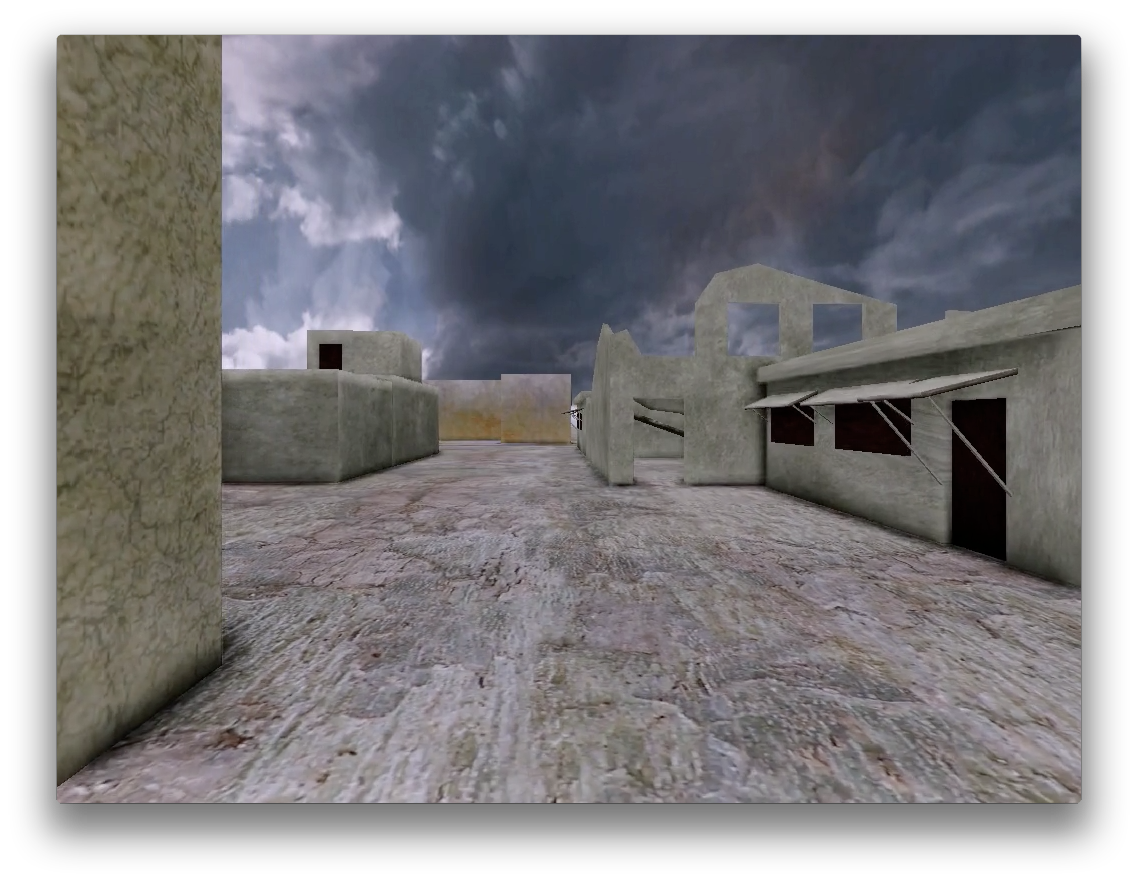
\includegraphics[width=\textwidth]{figures/stimulus-town}
\caption{}
\label{fig:stimulus-town}
\end{subfigure}
\begin{subfigure}{0.4\textwidth}
\centering
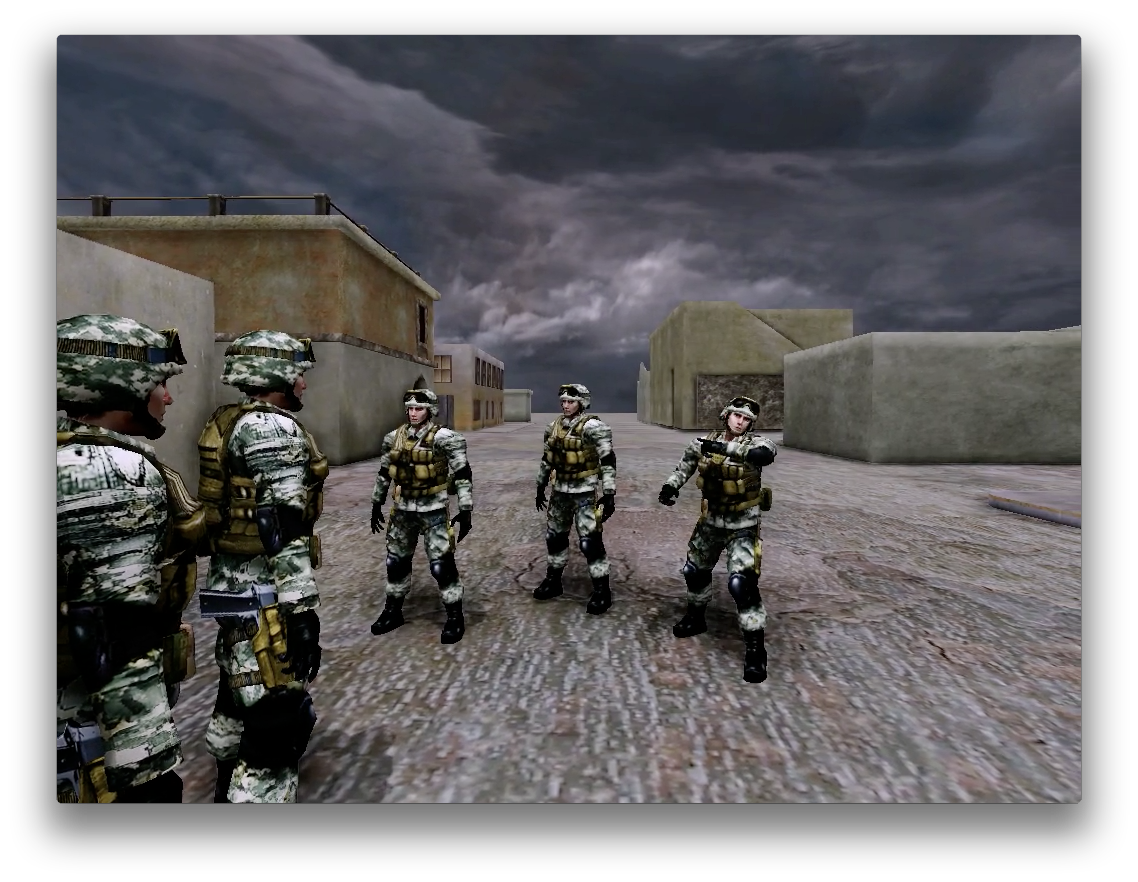
\includegraphics[width=\textwidth]{figures/stimulus-five-soldiers}
\caption{}
\label{fig:stimulus-five-soldiers}
\end{subfigure}
\begin{subfigure}{0.4\textwidth}
\centering
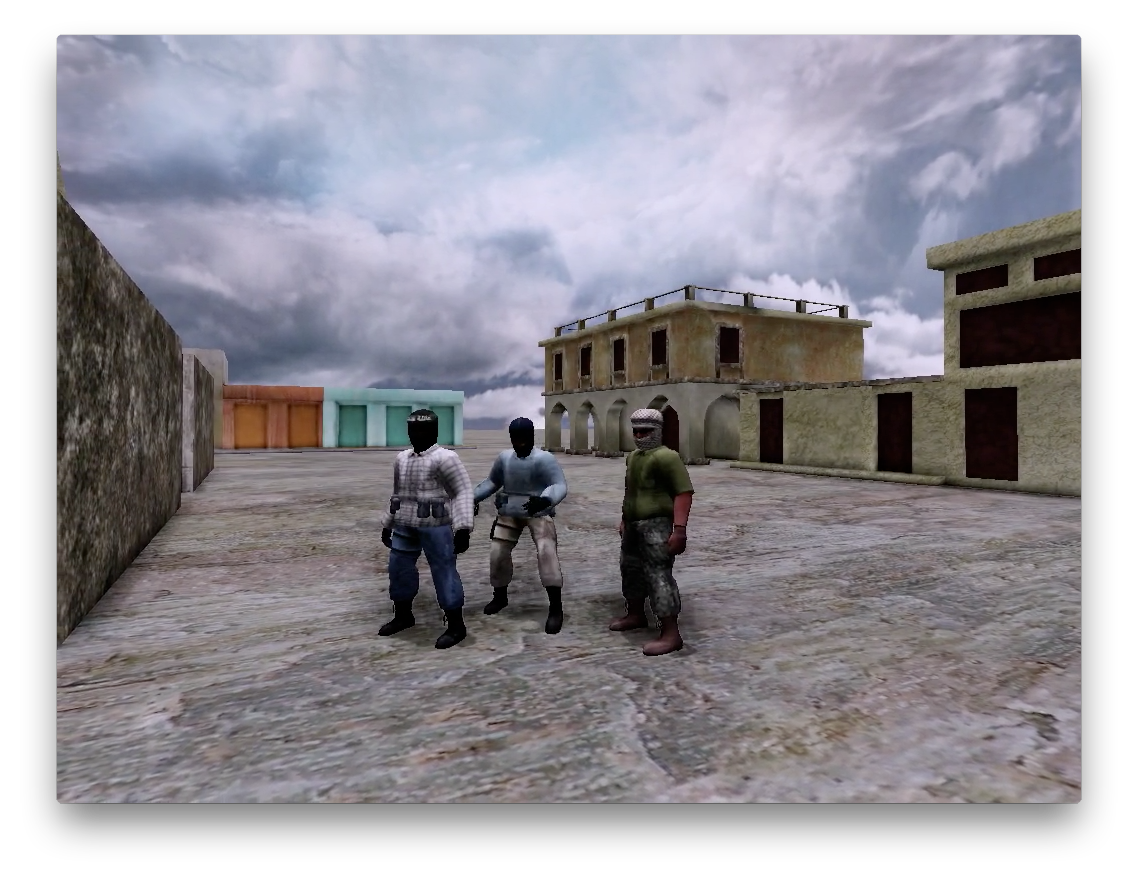
\includegraphics[width=\textwidth]{figures/stimulus-three-insurgents}
\caption{}
\label{fig:stimulus-three-insurgents}
\end{subfigure}
\caption{
\subref{fig:stimulus-town} An example frame from the stimulus where the camera is travel through the virtual envronment with no charcters presented.
\subref{fig:stimulus-five-soldiers} An example frame from the stimulus while characters are being presented.
\subref{fig:stimulus-three-insurgents} Another example frame from the stimulus while characters are being presented.
Note how the locations of the characters varies considerably between these two frames.}
\label{fig:stimulus}
\end{figure}

Scanning sessions included 5--6 six-min-duration runs,
each containing 12 alternations between moving through the virtual environment and character presentations. 
The number of characters presented in each block varied from 1 to 6.
A presentation with a particular number of characters appears twice in each run; however, the order of these presentations was randomized.
This random ordering was generated once and repeated for each subject.
There were 4 locations in the town used for presenting characters, and a single run made 3 loops through the town.
The order of presentation was chosed such that configurations with the same number of characters varied in location within the town; compare figures \ref{fig:stimulus-characters} and \ref{fig:stimulus-location}.
A single type of character (friends or foes) was presented in each run. Character type was randomly shuffled between runs.

\subsection{MRI protocols}
Imaging was performed an GE Signa Excite HD scanner using the product 8-channel head coil.
We collected whole-brain image volumes using a custom GRAPPA-accelerated EPI sequence \citep{newbold}. 
Sequence parameters were g-factor = 2,  TE = 25 ms, TR = 2.5 s, and  2.5-mm cubic voxels across a 200 mm field-of-view. 
The slice prescription included 40 slices oriented along the AC-PC axis. 
A high-order shim was  performed to improve field homogeneity.

A set of T1-weighted structural images was obtained on the same prescription at the end of each machine-learning session using a three-dimensional (3D) fast RF-spoiled GRASS (fSPGR) sequence. 
These anatomical images were then used to align the functional data to a structural 3D reference volume, which was acquired for each subject in a separate session. 
The structural reference volume was T1-weighted with good gray-white contrast and was acquired using a 3D, inversion-prepared, fSPGR sequence (minimum TE and TR, TI = 450 ms, 15$^\circ$ flip angle, isometric voxel size of 0.7 mm, 2 excitations, $\sim$28-minute duration).

\subsection{Preprocessing}
Preprocessing of the fMRI data was performed using the mrVista software package (available for download at \url{http://vistalab.stanford.edu/}) as well as additional tools developed on the mrVista framework in our lab. 
The first 15 seconds of data  were discarded to reduce transient effects.
We then estimated in-scan motion using a robust scheme \citep{Nestares-and-Heeger-2000}. 
Between-run motion was corrected using the same intensity-based scheme, this time applied to the temporal average intensity of the entire scan. 
The first run of the session was used as the reference. 
Additionally, we applied a Wiener filter deconvolution \citep{Wiener} using a generic difference-of-gamma HRF \citep{Glover} to shift the peak response in time so that it is aligned with its associated stimulus.

Wiener filter deconvolution can be summarized as follows:
Given a system
\begin{equation}
y(t) = h(t) \ast x(t) + n(t)
\end{equation}
where $x(t)$ is the signal of interest, $h(t)$ is some blurring kernel, $n(t)$ is independent additive noise, and $y(t)$ is the recorded signal.
We want to find the deconvolution kernel $g(t)$ such that 
\begin{equation}
\hat{x}(t) = g(t) \ast y(t)
\end{equation}
minimizes the mean squared error between $x(t)$ and $\hat{x}(t)$, or
\begin{equation}
\sum_{t}{\left( \hat{x}(t) - x(t) \right)^{2}}
\end{equation}
The solution for the optimal $g(t)$ is most easily expressed in the Fourier domain.
\begin{equation}
g(t) \xrightarrow{\mathcal{F}} \frac{H^{*}(f)}{\left|H(f)^{2}\right| + \mbox{SNR}^{-1}(f)}
\end{equation}
Where $\mbox{SNR}(f)$ is the signal to noise ratio $\frac{\left| X(f) \right|}{\left| N(f) \right|}$.

In fMRI, $y(t)$ is the recorded BOLD signal, $h(t)$ is the hemodynamic response function, and $x(t)$ is the neural response.
Calculating $g(t)$ requires estimates of the power spectral density of the signal of interest as well as the noise.
However, the noise $n(t)$ corresponds not only to scanner noise but other nuisance factors such as pulse and respiration.
This makes modeling the noise, and its power spectral density, very difficult.
Therefore, we set $\mbox{SNR}(f) = 1$ for all frequencies $f$.
Figure \ref{fig:wiener-deconvolution} illustrates the effects of this deconvolution on a simple square wave as well as an example voxel time series.

\begin{figure}
\centering
\begin{subfigure}{0.4\textwidth}
\centering
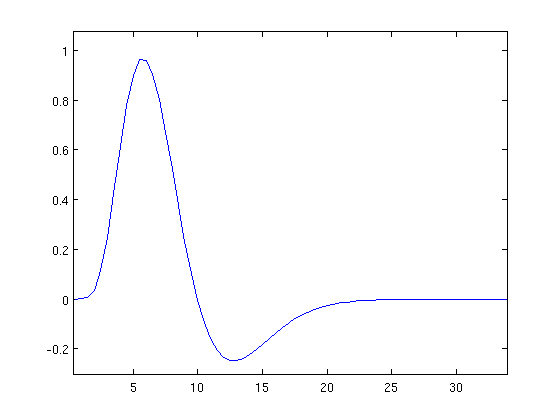
\includegraphics[width=\textwidth]{figures/hrf}
\caption{}
\label{fig:wiener-hrf}
\end{subfigure}
\begin{subfigure}{0.4\textwidth}
\centering
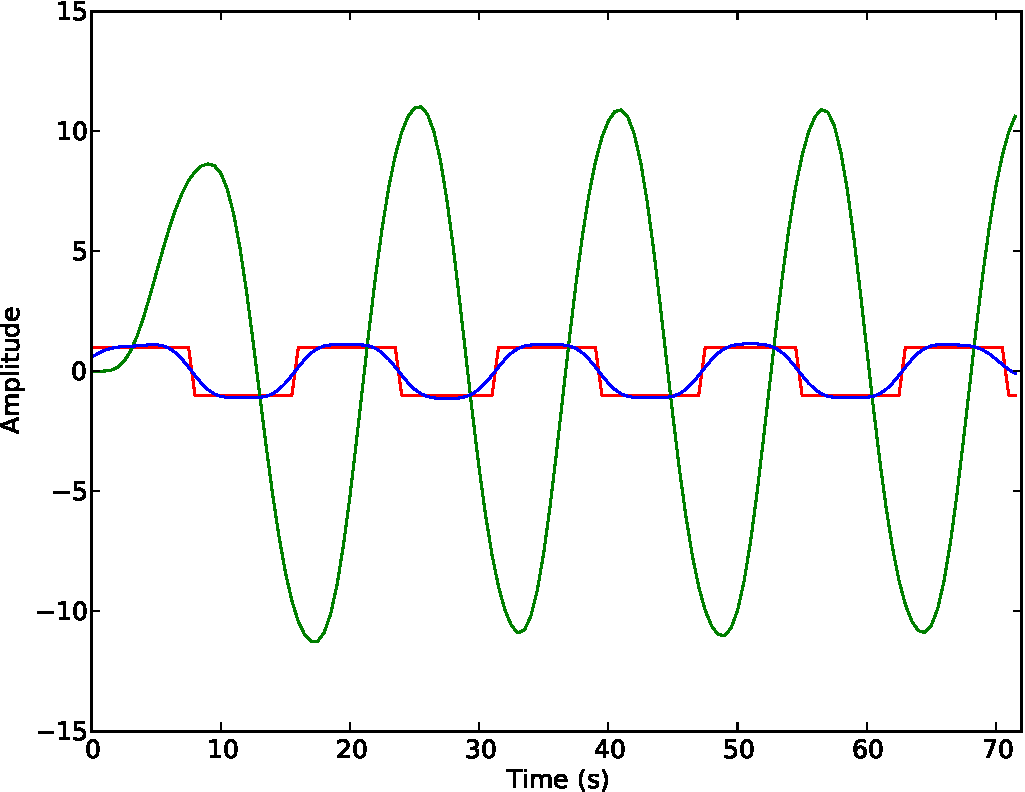
\includegraphics[width=\textwidth]{figures/square-wiener-deconvolution}
\caption{}
\label{fig:wiener-square}
\end{subfigure}
\begin{subfigure}{0.4\textwidth}
\centering
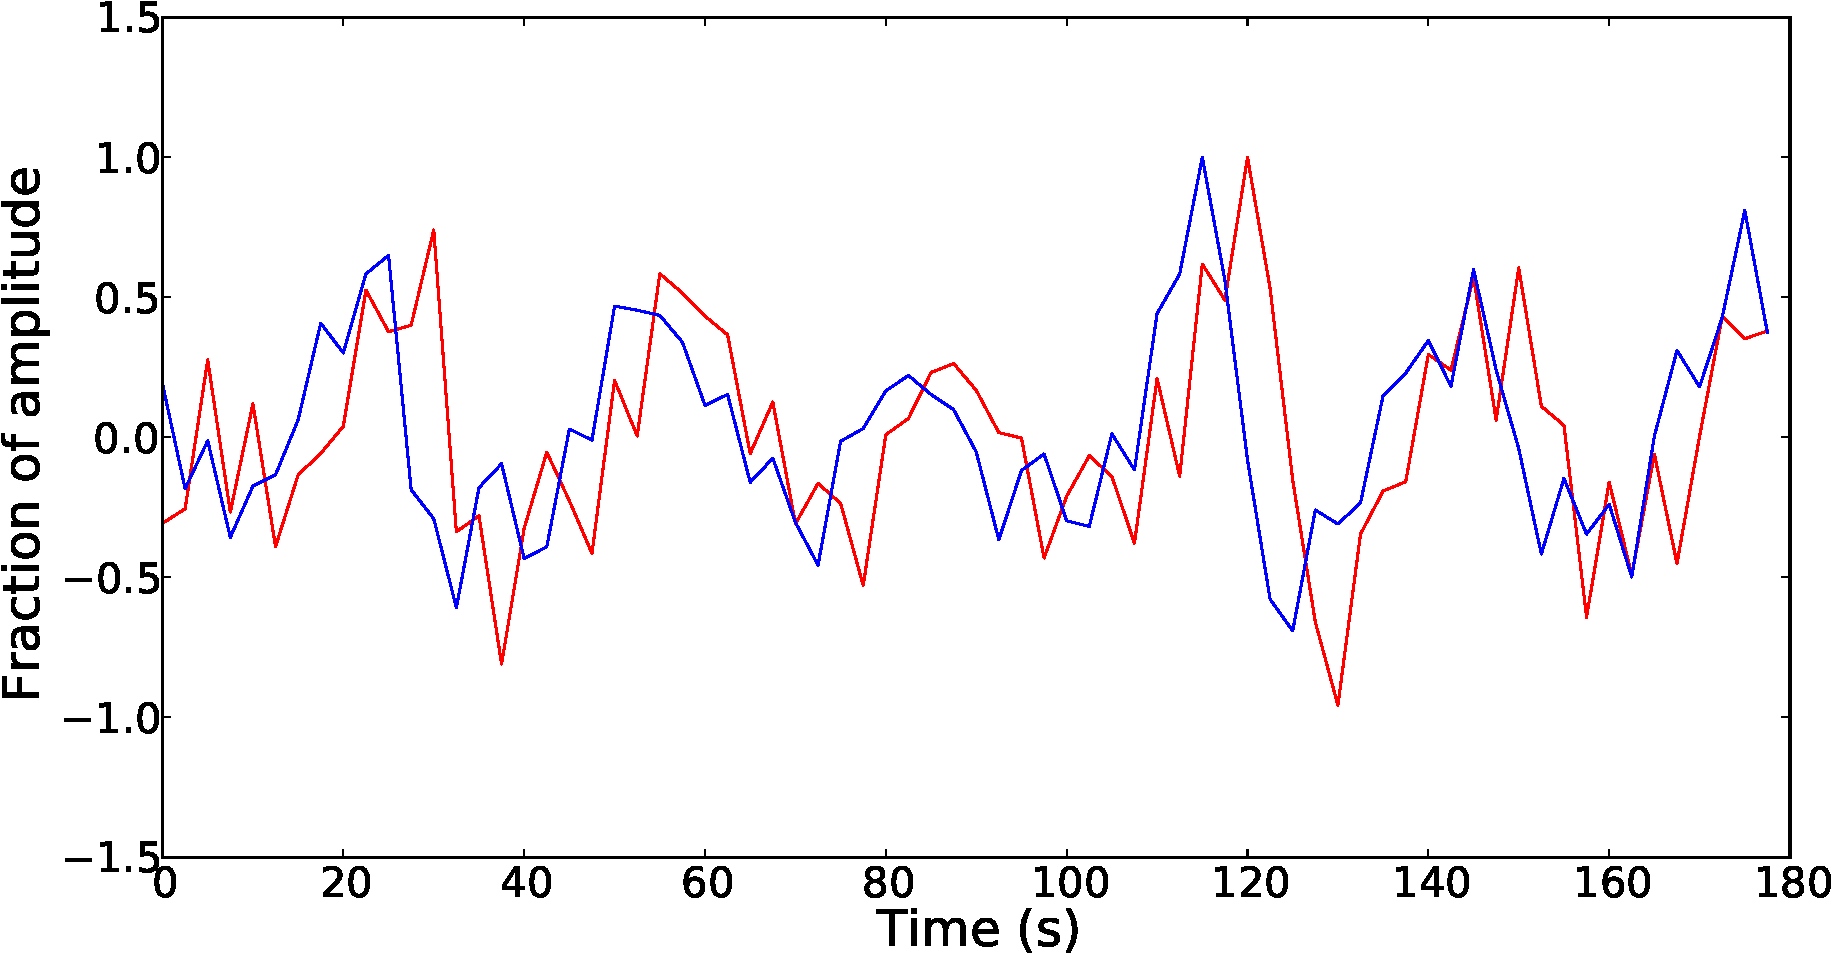
\includegraphics[width=\textwidth]{figures/voxel-wiener-deconvolution}
\caption{}
\label{fig:wiener-voxel}
\end{subfigure}
\caption{
\subref{fig:wiener-hrf} The difference-of-gamma HRF employed as $h(t)$. 
\subref{fig:wiener-square} A simple square wave in red. 
The same square wave after convolution with $h(t)$ in green, then after Wiener-filter deconvolution in blue. 
\subref{fig:wiener-voxel} An example voxel time series in red. 
The same time series after Wiener-filter deconvolution in blue.}
\label{fig:wiener-deconvolution}
\end{figure}

The high-resolution reference anatomies were segmented using the FreeSurfer analysis package \citep{FreeSurfer} to create approximate masks of the gray matter in each subject, as well as a surface model useful for visualization of the results.

\subsection{Dimensionality reduction}
Each voxel can be thought of as corresponding to a separate dimension of a very high dimenional space.
In our case, the number of voxels/dimensions was typically 80 x 80 x 40 = 256,000.
An important first step performed for most all machine learning algorithms is to reduce the total amount of data fed into the algorithms.
This not only speeds up the algorithm, but if done carefully, can improve the performance of the resulting classifiers.

In our case, we select voxels that are driven most strongly by the 30-sec duty cycle of our block design
using a harmonic power analysis technique. 
One can show that the response of any linear system to a blocked alternation at frequency $f$ will contain power only at $f$ and its harmonics. 
Under a linear response assumption, we can therefore form an unbiased estimate of the response power by summing the power at these frequencies. 
Let $y(t)$ be the recorded discrete time series at some voxel.
Then let $Y(f)$ be the discrete Fourier transform of $y(t)$.
The fractional harmonic power of that time series is defined as:
\begin{equation}
P_h = \frac{\sum_{i = 1}^{M}{\left|Y(i \cdot N)\right|^{2}}}{\sum_{f}{\left|Y(f)\right|^{2}}}
\end{equation}
Where $P_h$ is the fractional harmonic power, $M$ is the number of harmonics, and $N$ is the frequency of interest, in our case the period of the block alternations. 
Because the BOLD response has a predominantly low-pass temporal frequency response, we can accept $M = 4$. 
Using $P_h$, we then selected a particular number $N$ (typically 2000) voxels with the greatest power. 

This harmonic-power selection was based on the alternation between characters present and characters absent, without regard to the number of characters presented. 
Therefore, we will only be presenting classifier accuracy estimates for character count, and not for the presence or absence of characters to avoid cross-contamination between dimension-reduction and  classification criteria that would result in inflated classifier performance estimates \citep{CrossContamination}.
However, as a check we built classifiers to distinguish between time points with and without characters, and their performance was consistently above 95\%, confirming the proper operation of our machine-learning algorithms.

\subsection{Classification}
Using the time series from the voxels selected by the harmonic power analysis, we trained a linear SVM and a feed forward neural network.
Generally, the performance of machine learning algorithms is estimated by splitting the available data into a training set and a test set and then evaluating the performance of the algorithm on the test set after ``training" the model using only the training set \citep{needRef1}.
The idea is that the algorithm's performance on the test set is an estimate of the classifier's performance on new data gathered at a different time.
Neural network machine learning algorithms, further subdivide the data into training, validation, and test sets.
The algorithm is trained on the training set and after each iteration is evaluated with the validation set.
When the performance on validation set stops improving, the algorithm stops iterating; this procedure avoids so-called ``over fitting" of the data.
Performance of the resulting classifier is then evaluated on the test set in order to estimate its future performance \citep{needRef2}.

\emph{The above paragraph needs a couple of elementary references on machine-learning approaches.}

We estimated the performance of our algorithms using a cross-fold approach \citep{Kohavi1995} where the data is split into ``folds" that are used to form multiple training and test sets.
To maximize our temporal resolution, each ``frame" (time point) was treated as a separate distinct data value, rather than performing averaging across the 15-sec block as has been done in previous work \citep{BlockAveraging}.
Since each frame is 2.5 sec., averaging would have replaced 15sec/2.5sec. = 6 samples with a single averaged sample, unnecessarily reducing the temporal resolution by a factor of 6.

Previous studies have discussed issues with optimistically biased performance estimates due to temporal correlations violating independence assumptions between training and test set samples \citep{Pereira2009}. The slow speed of the fMRI hemodynamic response clearly introduces temporal correlations on time scales less than 15 seconds.
For our data, artificial correlations occur when the random sampling that divides the data into the different sets yields training and test samples from the same (15 sec.) block.

This raises a more general question: what is the relationship between performance estimates and temporal correlation?
To explore this, we estimated classifier performance using 5 different methods for splitting the training and test examples in order to vary the average temporal distance between frames in the two sets. 
The first four methods deal only with frames from a particular session.
In the first method, which we will refer to as  ``frame split", frames were independently drawn into the training and test sets. 
Although the draws were independent, there is no restriction to prevent adjacent frames being split between the training and test sets.We expect this method to exhibit artificially high performance because of the aforementioned temporal correlation of the slow fMRI data.
In the second method, which we will refer to as ``block split", sets of frames corresponding to the 15 sec. blocks were independently drawn into the training and test sets.
In our third method, we exploit the fact that each 6 min run cycles through all combinations twice, but in a different order the second time.
Accordingly, sets of frames were independently drawn from these half-runs, refered to as ``half-run split". 
In our fourth method, termed ``run split", entire 6-min runs of frames were independently drawn. 
And finally, for the fifth method, termed ``session split", we used one entire session for training and a second session for test.
This method is similar to measures of between-session classifier accuracy used in \citep{BetweenSessionAccuracy}.
Table \ref{tab:training-split} summarizes these training and test set split methods and the mean temporal distance between the training and test data, which varies from $\sim$30 s (frame split) to several months (session split).

\begin{figure}
\centering
\begin{subfigure}{0.4\textwidth}
\centering
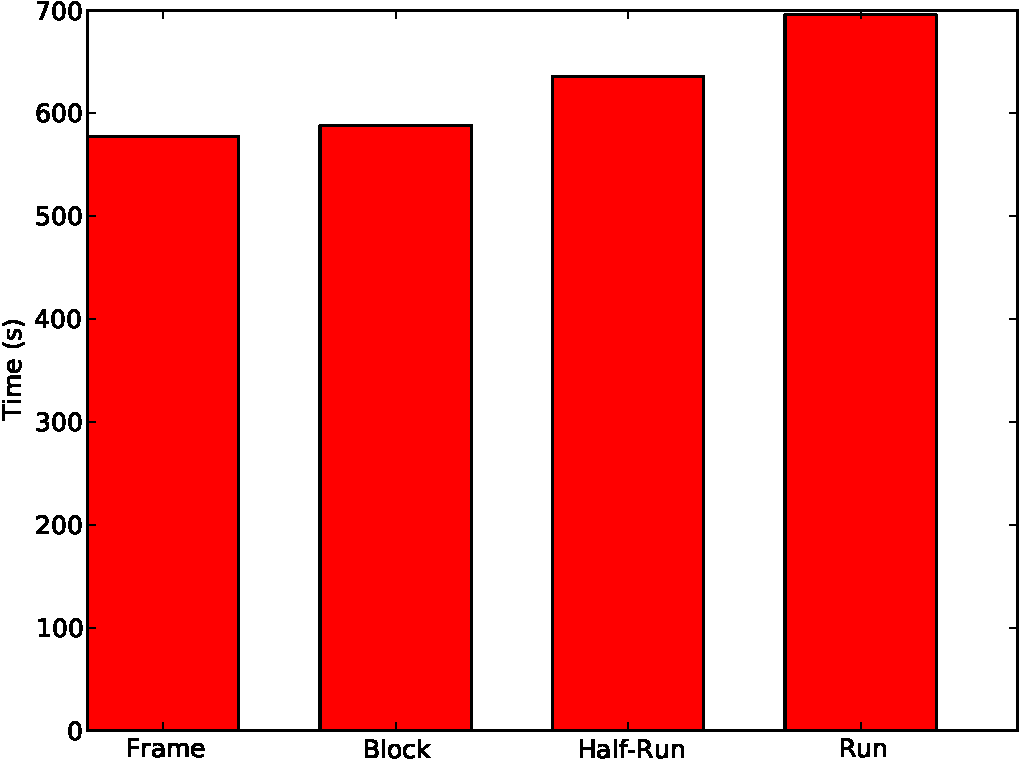
\includegraphics[width=\textwidth]{figures/mean-delay-graph}
\caption{}
\label{fig:mean-delay-graph}
\end{subfigure}
\begin{subfigure}{0.4\textwidth}
\centering
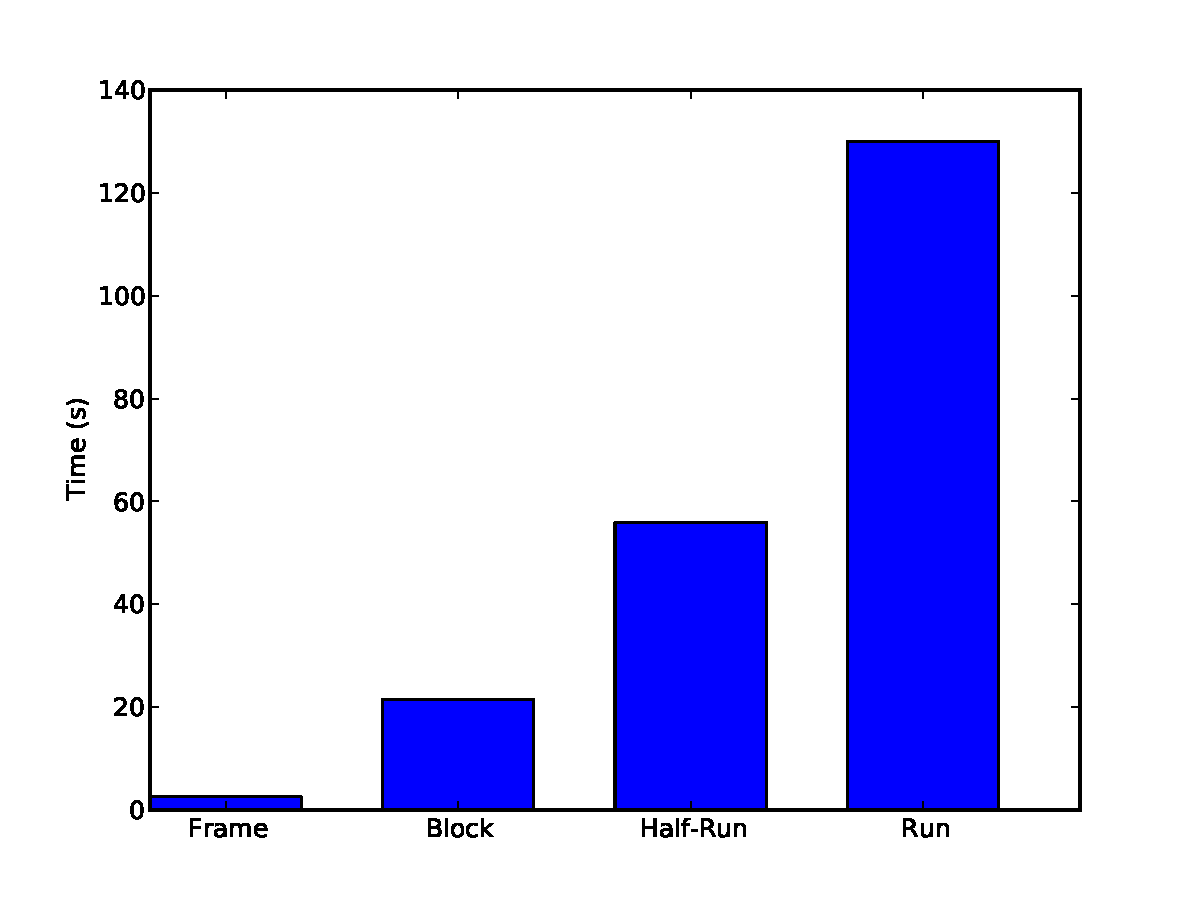
\includegraphics[width=\textwidth]{figures/min-delay-graph}
\caption{}
\label{fig:min-delay-graph}
\end{subfigure}
\caption{The \subref{fig:mean-delay-graph} mean delay and \subref{fig:min-delay-graph} minimum mean delay between examples in the train and test set for four of the split methods. 
The session split method is excluded because both the mean and minimum delay are much larger than the other splits and the delays vary significantly between subjects.}
\end{figure}

\begin{table}
\centering

\begin{tabular}{l*{2}{c}}
\toprule
Split & Mean Delay & Mean Minimum Delay \\
\midrule
Frame & 5776 & 26 \\
Block & 5883 & 215 \\
Half-Run & 6360 & 559 \\
Run & 6960 & 1300 \\
Session & 0 & 0 \\
\bottomrule 
\end{tabular}

\caption{Summary of training and test set split methods and the mean temporal delay between the training and test data.}
\label{tab:training-split}
\end{table}

For the frame and block splits, the classifier performances were estimated using 10-fold cross-validation.
That is, the dataset was randomly split into the training and test sets 10 times and a classifier is trained on each split.
The classifier's performance is then estimated as the average of its performance across all 10 splits.
For the half-run, run, and session splits, only 8, 4, and 2 unique splits are possible, respectively, due to the much smaller number of runs and sessions per subject. 
Therefore, only 8-fold, 4-fold, and 2-fold cross-validation were employed for estimating classifier performance on these splits.

We define the classifier's overall performance or accuracy to be the probability that it will correctly classify a previously unseen time-slice.
As such, this measure of performance can only be estimated by dividing the number of correctly classified examples in the test set by the total number of examples in the test set.
We can also discuss classifier performance with respect to a single class.
Single class performance is traditionally measured along two axes: \emph{precision} and \emph{recall}.
\emph{Precision} with respect to class $c$ is the probability that a previously unseen data point was classified correctly given that it was classified as $c$.
\emph{Recall} with respect to class $c$ is the probability that a previously unseen data point was classified correctly given that it is actually a member of $c$.
Again, these measures can only be estimated from the test set.
$\mbox{\emph{precision}} = tp / (tp + fp)$, where $tp$ is the number of true positives and $fp$ is the number of false positives.
$\mbox{\emph{recall}} = tp / (tp + fn)$, where $fn$ is the number of false negatives.

Another tool for examining classifier performance is the confusion matrix.
If $\mathbf{C}$ is a confusion matrix, then the value of $C_{ij}$ is equal to the number examples of class $i$ that were classified as class $j$.
Therefore, values along the diagonal of a confusion matrix correspond to correct classifications while other values correspond to incorrect classifications.
The confusion matrix also simplifies estimating precision and recall for each class.
The value of $C_{ii}$ divided by the sum of all values along row $i$ is the estimate for the recall of the $i^{th}$ class.
Similarly, the value of $C_{jj}$ divided by the sum of all values along column $j$ is the estimate for the precision of the $j^{th}$ class.
Finally, overall classifier performance can be estimated by dividing the sum along the diagonal, or the trace, by the sum of the entire matrix.

\subsection{Sensitivity Analysis}
Non-linear multi-variate machine-learning classifiers can tell us whether the time-series data from a subset of human brain voxels is discriminative with respect to the task being predicted. 
However, these results do not show which voxels in the large group were actually important for that discrimination.
This information is important for localizing functions in the brain.
One existing technique is to train machine learning classifiers on small localized areas in the brain and use their performance as a measure of the strength of the function in question in that area \citep{needRef3}.
While this technique is effective for simple highly localized functions, the results are less clear when the function is sparsely distributed over the brain.
No one region may contain enough information for accurate predictions.

To overcome this limitation, we have trained our classifiers on all stimulus-responsive regions of the brain and used a neural-network sensitivity analysis to display the spatially distributed set of voxels that are the most important for identifying the classes.
Specifically, we calculate the sensitivity, or magnitude of change, of the output of the classifier with respect to a change in each voxel
 \citep{Zurada1994}.
Let $\mathbf{o}$ be the vector of outputs and $\mathbf{x}$ be the vector of inputs.
Then the sensitivity of output $k$ to input $i$ is defined by:
\begin{equation}
S_{ki} = \frac{\delta o_{k}}{\delta x_{i}}
\end{equation}
which is simply the partial derivative of the output with respect to the input.
If we let $\mathbf{w}$ be the weight matrix from the hidden layer to the output layer and $\mathbf{v}$ be the weight matrix from the input layer to the hidden layer then the partial derivative can be expressed as follows:
\begin{equation}
\frac{\delta o_{k}}{\delta x_{i}} = o'_{k} \sum^{J}_{j=1}{w_{kj}y'_{j}v_{ji}}
\end{equation}
Where $J$ is the total number of hidden neurons,  $o'_{k}$ is the value of the derivative of the activation function at output $k$, and $y'_{j}$ is the value of the derivative of the activation function at hidden neuron $j$.
Finally, the entire sensitivity matrix can be expressed in matrix notation as:
\begin{equation}
\mathbf{S} = \mathbf{O}' \times \mathbf{W} \times \mathbf{Y}' \times \mathbf{V}
\end{equation}
Where
\begin{equation}
\mathbf{O}' = diag(o'_{1},~o'_{2},~\cdots,~o'_{K})
\end{equation}
\begin{equation}
\mathbf{Y}' = diag(y'_{1},~y'_{2},~\cdots,~y'_{K})
\end{equation}
However, because the transfer functions are non-linear they can only be evaluated for specific input values.
Therefore, we calculate the average sensitivity matrix across all input vectors.
\begin{equation}
\mathbf{S}_{avg} = \sqrt{ \frac{ \sum_{n = 1}^{N}{ \left( \mathbf{S}^{n}\right)^{2} } }{N} }
\end{equation}
Where $N$ is the number of input vectors.
The magnitude is squared to avoid problems with positive and negative sensitivities canceling out when averaging.
The average of the absolute value of sensitivities could also be employed.
This still gives a sensitivity value for each voxel with respect to every output, whereas it is useful to have a measure of the sensitivity of a voxel with respect to any output.
To calculate this number, we simply take the maximum sensitivity of each voxel across all outputs.
\begin{equation}
\Phi_{i} = \max_{k=1 \dots K}{S_{ki,~avg}}
\end{equation}
This sensitivity can now be projected back into the volume anatomy space to create a sensitivity map that reflects the relative incremental importance of each voxel's response to the classification decision.
Further, we used this sensitivity analysis to further reduce the dimensionality of the neural network by retraining the algorithm using only the voxels that had a sensitivity over some threshold.
This threshold was determined by iteratively retraining the neural network with successively higher thresholds until the performance of the classifier began to degrade.

We employed FreeSurfer \citep{FreeSurfer} to construct cortical surfaces for each of our subjects using the previously collected high resolution anatomy volumes.
Then, we constructed 10 anatomical labels on each surface based on FreeSurfer's automatically generated labels.
These labels are presented in figure \ref{fig:labels}.
The labels we used largely overlap with FreeSurfer's labels.
However, the label for the banks of the superior temporal sulcus was subdivided and incorporated back in to the superior and middle temporal labels.
Additionally, the supramarginal label was merged with the inferior parietal label.
For most subjects, several of the automatic labels were also edited by hand to better conform with the sulcal boundaries of the subject.
We then projected each subject's volume sensitivity map onto their cortical surface and blurred along the surface using a five millimeter full-width half-maximum (FWHM) Gaussian kernel.

\begin{figure}
\centering
\begin{subfigure}{0.4\textwidth}
\centering
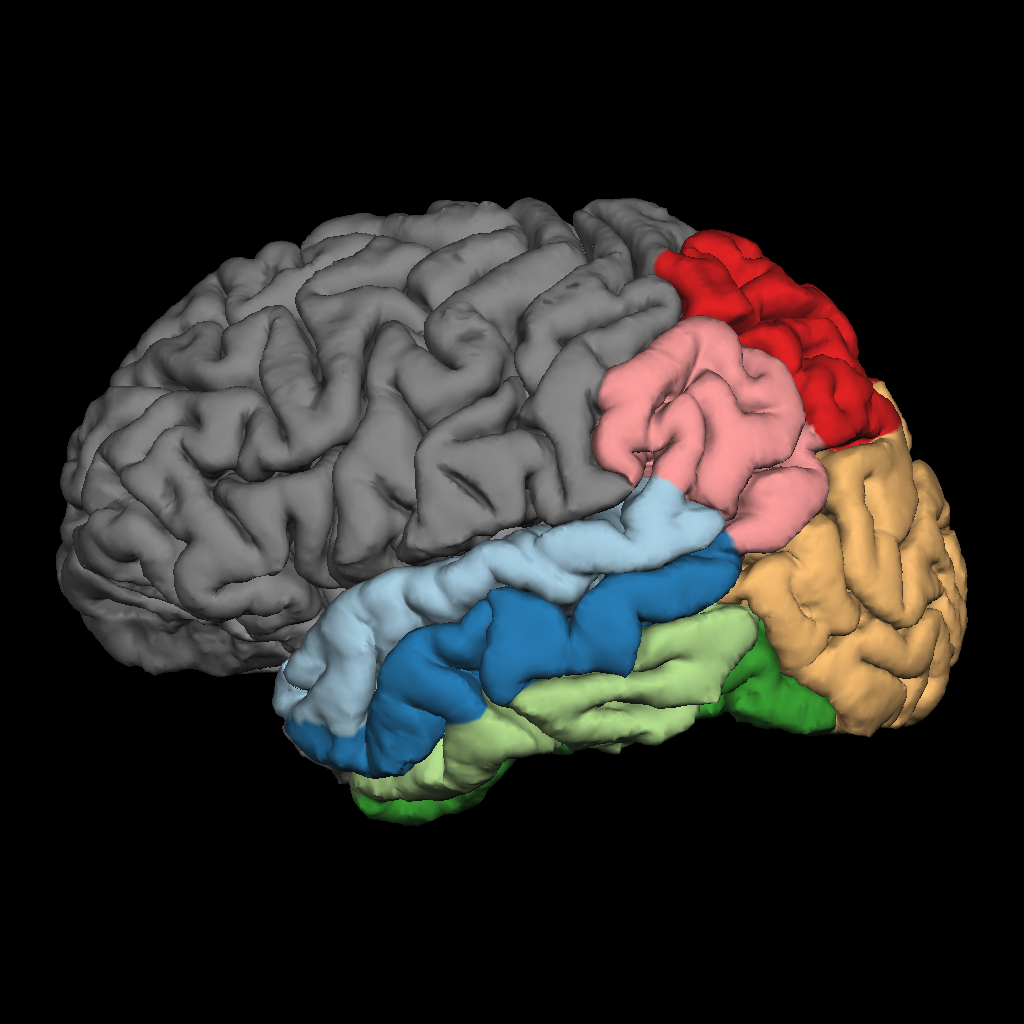
\includegraphics[width=\textwidth]{figures/lh-lateral-labels}
\caption{lateral labels}
\label{fig:leteral-labels}
\end{subfigure}
\begin{subfigure}{0.4\textwidth}
\centering
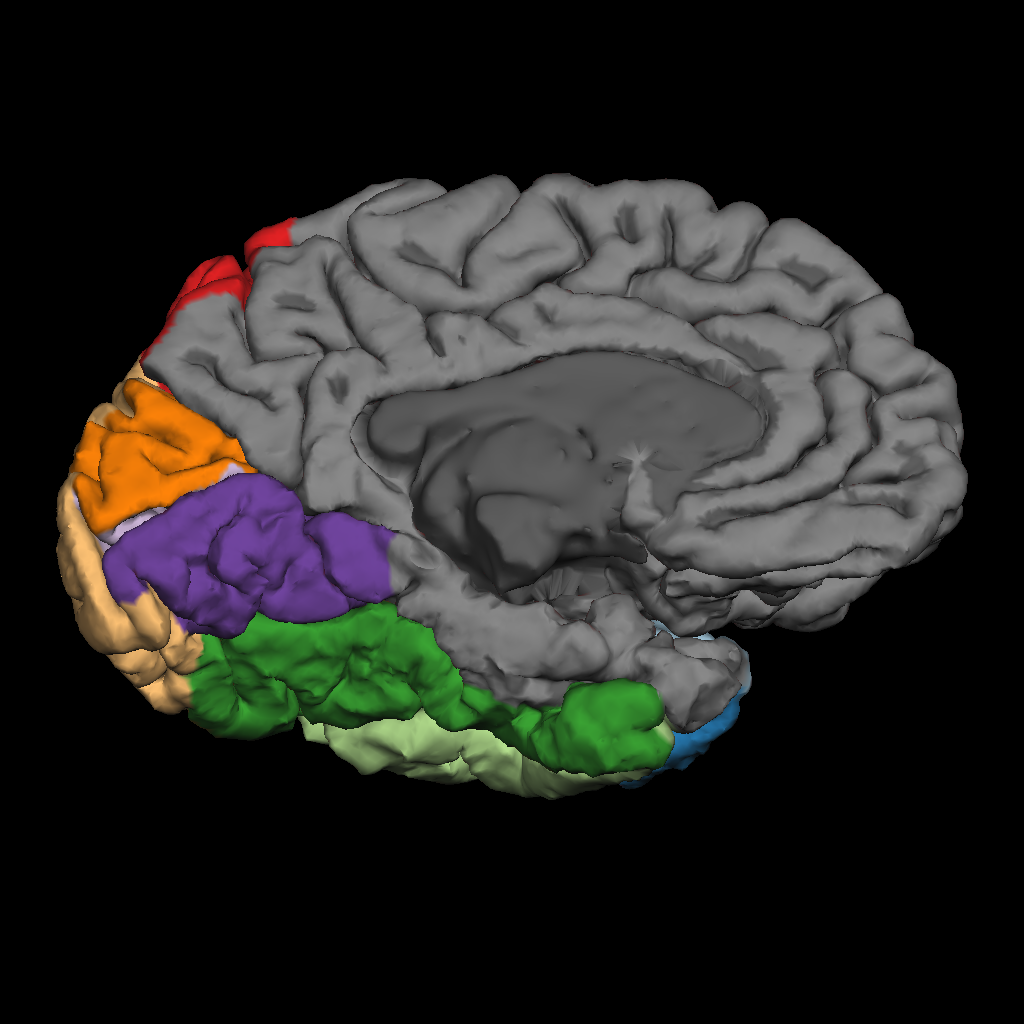
\includegraphics[width=\textwidth]{figures/lh-medial-labels}
\caption{medial labels}
\label{fig:medial-labels}
\end{subfigure}
\caption{Color coded region labels used for aggregating sensitivity results: light blue -- superior temporal, dark blue -- middle temporal, light green -- inferior temporal, dark green -- fusiform, dark red -- superior perietal, light red -- inferior parietal, light orange -- lateral occipital, dark orange -- cuneus, light purple -- pericalcarine, dark purple -- lingual}
\end{figure}

\section{Results}
Table \ref{tab:results} contains the cross-validated performance estimates of the linear SVM and feed forward neural networks for all five subjects and all five training and test split methods.
There is some variation of classifier performance between subjects, but in all cases the performance is significantly ($p < 0.001$) above chance. 

\begin{figure*}
\centering
\begin{subfigure}{0.8\textwidth}
\centering
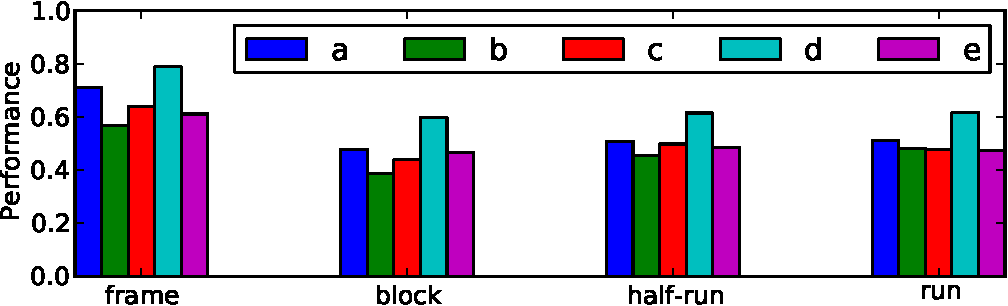
\includegraphics[width=\textwidth]{figures/svm-performance-graph}
\caption{}
\label{fig:svm-performance-graph}
\end{subfigure}
\begin{subfigure}{0.8\textwidth}
\centering
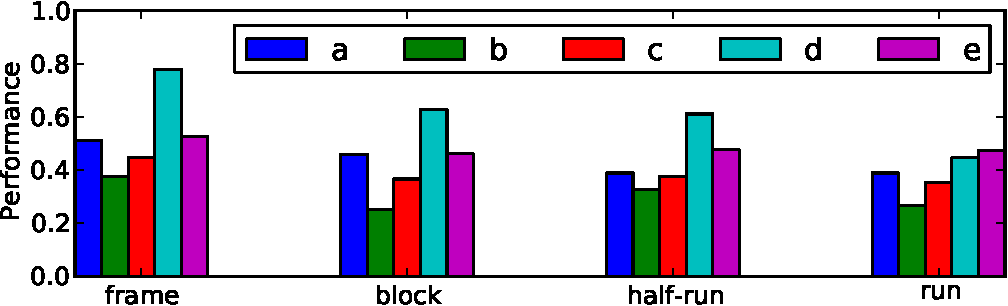
\includegraphics[width=\textwidth]{figures/nn-performance-graph}
\caption{}
\label{fig:nn-performance-graph}
\end{subfigure}
\caption{The performance estimates of the \subref{fig:svm-performance-graph} linear SVM and the \subref{fig:nn-performance-graph} feedforward neural network after cross-validation for all five subjects and four of the training and test split methods. }
\end{figure*}

It is evident that, as the average temporal delay between data in the training and test sets increases, the estimated performance of the classifiers decreases.
This relationship is plotted in figure \ref{fig:performance-verse-temporal-distance}.

\begin{figure}
\centering
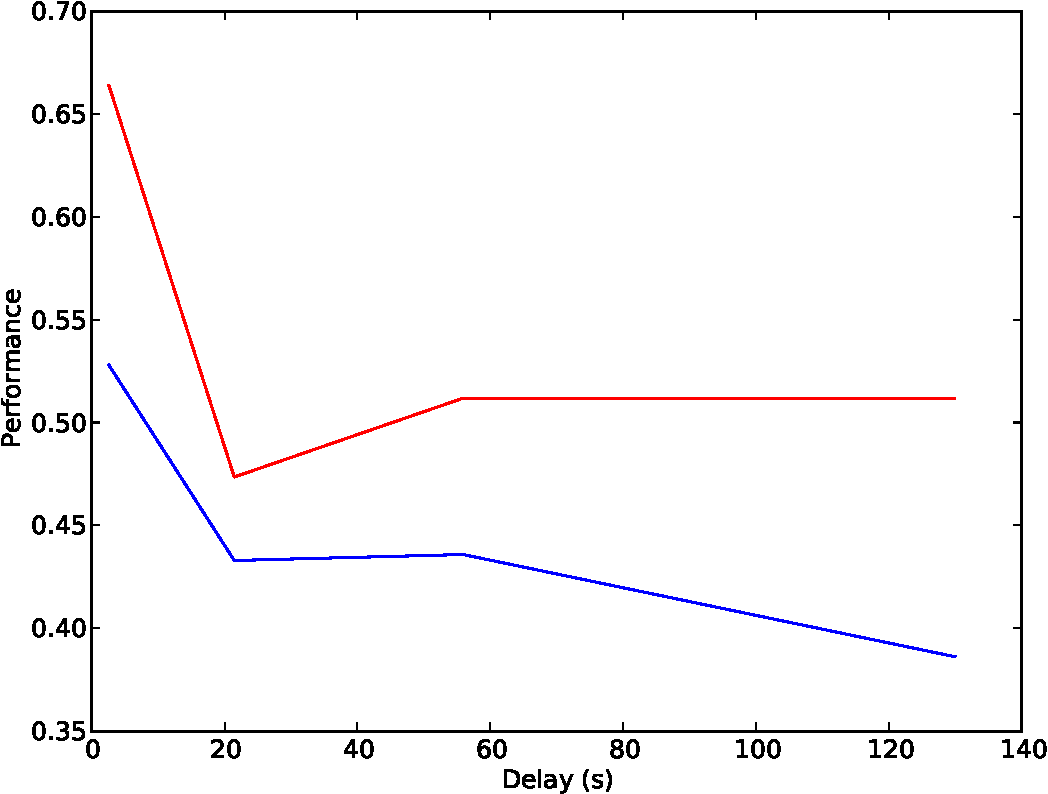
\includegraphics[width=0.4\textwidth]{figures/performance-verse-temporal-distance}
\caption{The average performance of the SVM and neural network classifiers plotted against the average temporal delay between data in the training and test sets.}
\label{fig:performance-verse-temporal-distance}
\end{figure}

The average confusion matrix presented in figure \ref{fig:average-confusion} gives a more intuitive look at the performance of the classifier.
From this matrix we can see that the classifiers are much better at detecting the presence of a single character than any other count.
In fact, there are almost no cases of confusion between 1 and 2 characters.
Apparently, these two situations evoke very different responses in the brain.
The rest of the character counts are distinguished with relatively equal accuracy,
except for a slightly larger tendency to mis-classify the 6 character presentation.
It should also be noted that the majority of the incorrect responses lay just off the main diagonal.
These responses correspond to the classifier being wrong by a single character in its classification.
For example, the machine learning algorithm classified a frame as containing 4 characters when it only contained 3 characters.
The estimated performance does not take the cardinality of the classes into account and considers mislabeling 1 character as 2 equivalent to mislabeling 1 character as 6 characters.
A soft measure of accuracy that takes the cardinality of the classes into consideration may be useful but the results are harder to interpret.
A confusion matrix gives us the advantages of the soft measure while providing an easily interpretable look into the performance of the classifiers.

\begin{figure}
\centering
\begin{subfigure}{0.4\textwidth}
\centering

\begin{tabular}{*{9}{c}}
& & \multicolumn{6}{c}{predicted count} & \\
& & 1 & 2 & 3 & 4 & 5 & 6 & \\
\multirow{6}{*}{\begin{sideways}actual count\end{sideways}}
& 1 & \cellcolor[rgb]{0.000000,1.000000,0.000000}75\% & \cellcolor[rgb]{0.987315,0.012685,0.000000}6\% & \cellcolor[rgb]{0.967214,0.032786,0.000000}8\% & \cellcolor[rgb]{0.995154,0.004846,0.000000}3\% & \cellcolor[rgb]{0.996400,0.003600,0.000000}3\% & \cellcolor[rgb]{0.991856,0.008144,0.000000}5\% & \cellcolor[rgb]{0.000000,1.000000,0.000000}71\%\\
& 2 & \cellcolor[rgb]{0.984543,0.015457,0.000000}6\% & \cellcolor[rgb]{0.000001,0.999999,0.000000}52\% & \cellcolor[rgb]{0.960568,0.039432,0.000000}9\% & \cellcolor[rgb]{0.793233,0.206767,0.000000}13\% & \cellcolor[rgb]{0.989269,0.010731,0.000000}5\% & \cellcolor[rgb]{0.754492,0.245508,0.000000}14\% & \cellcolor[rgb]{0.000002,0.999998,0.000000}50\%\\
& 3 & \cellcolor[rgb]{0.976984,0.023016,0.000000}7\% & \cellcolor[rgb]{0.946464,0.053536,0.000000}9\% & \cellcolor[rgb]{0.000000,1.000000,0.000000}53\% & \cellcolor[rgb]{0.228780,0.771220,0.000000}20\% & \cellcolor[rgb]{0.980048,0.019952,0.000000}7\% & \cellcolor[rgb]{0.995294,0.004706,0.000000}3\% & \cellcolor[rgb]{0.000001,0.999999,0.000000}51\%\\
& 4 & \cellcolor[rgb]{0.992536,0.007464,0.000000}4\% & \cellcolor[rgb]{0.888490,0.111510,0.000000}11\% & \cellcolor[rgb]{0.154156,0.845844,0.000000}21\% & \cellcolor[rgb]{0.000336,0.999664,0.000000}37\% & \cellcolor[rgb]{0.500333,0.499667,0.000000}17\% & \cellcolor[rgb]{0.939464,0.060536,0.000000}10\% & \cellcolor[rgb]{0.000499,0.999501,0.000000}36\%\\
& 5 & \cellcolor[rgb]{0.995930,0.004070,0.000000}3\% & \cellcolor[rgb]{0.976984,0.023016,0.000000}7\% & \cellcolor[rgb]{0.934220,0.065780,0.000000}10\% & \cellcolor[rgb]{0.299381,0.700619,0.000000}19\% & \cellcolor[rgb]{0.000001,0.999999,0.000000}50\% & \cellcolor[rgb]{0.919415,0.080585,0.000000}11\% & \cellcolor[rgb]{0.000000,1.000000,0.000000}55\%\\
& 6 & \cellcolor[rgb]{0.917261,0.082739,0.000000}11\% & \cellcolor[rgb]{0.217071,0.782929,0.000000}20\% & \cellcolor[rgb]{0.994473,0.005527,0.000000}4\% & \cellcolor[rgb]{0.888730,0.111270,0.000000}11\% & \cellcolor[rgb]{0.880363,0.119637,0.000000}12\% & \cellcolor[rgb]{0.000031,0.999969,0.000000}43\% & \cellcolor[rgb]{0.000004,0.999996,0.000000}48\%\\
&   & \cellcolor[rgb]{0.000000,1.000000,0.000000}75\% & \cellcolor[rgb]{0.000001,0.999999,0.000000}52\% & \cellcolor[rgb]{0.000000,1.000000,0.000000}53\% & \cellcolor[rgb]{0.000336,0.999664,0.000000}37\% & \cellcolor[rgb]{0.000001,0.999999,0.000000}50\% & \cellcolor[rgb]{0.000031,0.999969,0.000000}43\% & \cellcolor[rgb]{0.000001,0.999999,0.000000}52\%\\
\end{tabular}

\caption{}
\label{fig:average-confusion-svm}
\end{subfigure}
\begin{subfigure}{0.4\textwidth}
\centering

\begin{tabular}{*{8}{c}}
& & \multicolumn{6}{c}{predicted count} \\
& & 1 & 2 & 3 & 4 & 5 & 6 \\
\multirow{6}{*}{\begin{sideways}actual count\end{sideways}}
& 1 & \cellcolor[rgb]{0.000000,1.000000,0.000000}62\% & \cellcolor[rgb]{0.975443,0.024557,0.000000}7\% & \cellcolor[rgb]{0.841309,0.158691,0.000000}12\% & \cellcolor[rgb]{0.971887,0.028113,0.000000}8\% & \cellcolor[rgb]{0.997938,0.002062,0.000000}1\% & \cellcolor[rgb]{0.960675,0.039325,0.000000}9\%\\
& 2 & \cellcolor[rgb]{0.933406,0.066594,0.000000}10\% & \cellcolor[rgb]{0.000009,0.999991,0.000000}46\% & \cellcolor[rgb]{0.933406,0.066594,0.000000}10\% & \cellcolor[rgb]{0.831816,0.168184,0.000000}13\% & \cellcolor[rgb]{0.989177,0.010823,0.000000}5\% & \cellcolor[rgb]{0.569328,0.430672,0.000000}16\%\\
& 3 & \cellcolor[rgb]{0.979969,0.020031,0.000000}7\% & \cellcolor[rgb]{0.960675,0.039325,0.000000}9\% & \cellcolor[rgb]{0.000018,0.999982,0.000000}44\% & \cellcolor[rgb]{0.071219,0.928781,0.000000}23\% & \cellcolor[rgb]{0.984753,0.015247,0.000000}6\% & \cellcolor[rgb]{0.902345,0.097655,0.000000}11\%\\
& 4 & \cellcolor[rgb]{0.989896,0.010104,0.000000}5\% & \cellcolor[rgb]{0.919227,0.080773,0.000000}11\% & \cellcolor[rgb]{0.159047,0.840953,0.000000}21\% & \cellcolor[rgb]{0.001187,0.998813,0.000000}34\% & \cellcolor[rgb]{0.739428,0.260572,0.000000}14\% & \cellcolor[rgb]{0.586267,0.413733,0.000000}16\%\\
& 5 & \cellcolor[rgb]{0.990567,0.009433,0.000000}5\% & \cellcolor[rgb]{0.971887,0.028113,0.000000}8\% & \cellcolor[rgb]{0.933406,0.066594,0.000000}10\% & \cellcolor[rgb]{0.333341,0.666659,0.000000}18\% & \cellcolor[rgb]{0.000017,0.999983,0.000000}44\% & \cellcolor[rgb]{0.697341,0.302659,0.000000}15\%\\
& 6 & \cellcolor[rgb]{0.945244,0.054756,0.000000}10\% & \cellcolor[rgb]{0.811482,0.188518,0.000000}13\% & \cellcolor[rgb]{0.937595,0.062405,0.000000}10\% & \cellcolor[rgb]{0.667251,0.332749,0.000000}15\% & \cellcolor[rgb]{0.902345,0.097655,0.000000}11\% & \cellcolor[rgb]{0.000049,0.999951,0.000000}41\%\\
\end{tabular}

\caption{}
\label{fig:average-confusion-nn}
\end{subfigure}
\caption{The average confusion matrices for the \subref{fig:average-confusion-svm} SVM and \subref{fig:average-confusion-nn} NN across all subjects using the block split.}
\label{fig:average-confusion}
\end{figure}

Sensitivity maps show a preponderance of brain activity in posterior parietal lobe, lateral occipital areas, and dorsal early extrastriate visual areas \ref{fig:ExampleSubjects}. Individual subjects also displayed small regions of high sensitivity in idiosyncratic portions of temporal frontal cortex. After aligning all of the subjects to the MNI template \ref{MNI} and combining these sensitivity maps, we find that classifier decisions were heavily dependent on activity in occipital and parietal lobes \ref{fig:MNI-average-sensitivity}.  Classifier sensitivity was most affect by, in order of importance, dorsal parietal lobe, cuneus, and lateral occipital regions \ref{sensitivityTable}. 

\begin{figure*}
\centering

\begin{tabular}{cccccccc}
\toprule
Region & A & B & C & D & E  & Mean & Confidence Interval\\
\midrule
right lateral occipital & 26.54 & 13.41 & 16.26 & 24.17 & 26.49 & 21.37 & 18.76--23.98 \\
left lateral occipital & 13.37 & 25.65 & 15.37 & 24.02 & 25.75 & 20.83 & 18.37--23.28 \\
left superior parietal & 3.36 & 0.33 & 3.66 & 3.85 & 6.11 & 3.46 & 2.76--4.26 \\
left inferior parietal & 2.88 & 5.43 & 7.08 & 5.47 & 5.36 & 5.24 & 4.73--5.78 \\
right lingual & 6.64 & 5.96 & 10.30 & 5.88 & 5.25 & 6.81 & 5.93--7.69 \\
right superior parietal & 3.12 & 5.98 & 2.54 & 7.14 & 4.87 & 4.73 & 3.93--5.53 \\
right inferior parietal & 1.76 & 6.96 & 0.81 & 1.68 & 4.56 & 3.16 & 2.12--4.21 \\
left pericalcarine & 7.07 & 0.29 & 2.29 & 3.79 & 3.87 & 3.46 & 2.45--4.49 \\
left lingual & 8.63 & 8.38 & 10.09 & 4.92 & 3.50 & 7.10 & 6.07--8.37 \\
right superior temporal & 0.91 & 0.83 & 0.98 & 2.18 & 2.62 & 1.50 & 1.16--1.85 \\
right middle temporal & 0.23 & 0.84 & 6.08 & 1.69 & 2.54 & 2.28 & 1.28--3.27 \\
right pericalcarine & 4.64 & 5.99 & 6.02 & 0.40 & 2.20 & 3.85 & 2.82--4.91 \\
left superior temporal & 3.15 & 0.00 & 1.72 & 2.17 & 1.82 & 1.77 & 1.34--2.23 \\
right fusiform & 2.43 & 3.42 & 3.19 & 3.51 & 1.42 & 2.79 & 2.43--3.17 \\
right cuneus & 0.77 & 4.89 & 1.36 & 0.12 & 1.24 & 1.68 & 0.86--2.51 \\
left cuneus & 2.60 & 4.15 & 2.11 & 0.13 & 0.85 & 1.97 & 1.31--2.63 \\
left inferior temporal & 0.04 & 0.00 & 0.46 & 0.66 & 0.83 & 0.40 & 0.24--0.55 \\
right inferior temporal & 3.65 & 1.44 & 0.96 & 3.43 & 0.64 & 2.02 & 1.43--2.58 \\
left fusiform & 2.67 & 1.12 & 6.24 & 4.48 & 0.08 & 2.92 & 1.89--3.94 \\
left middle temporal & 5.53 & 4.93 & 2.51 & 0.33 & 0.00 & 2.66 & 1.62--3.70 \\
\bottomrule
\end{tabular}

\caption{Sensitivity values integrated across cortical surface labels.}
\label{tab:full-sensitivity}
\end{figure*}

\begin{figure*}
\centering
\begin{subfigure}{0.4\textwidth}
\centering
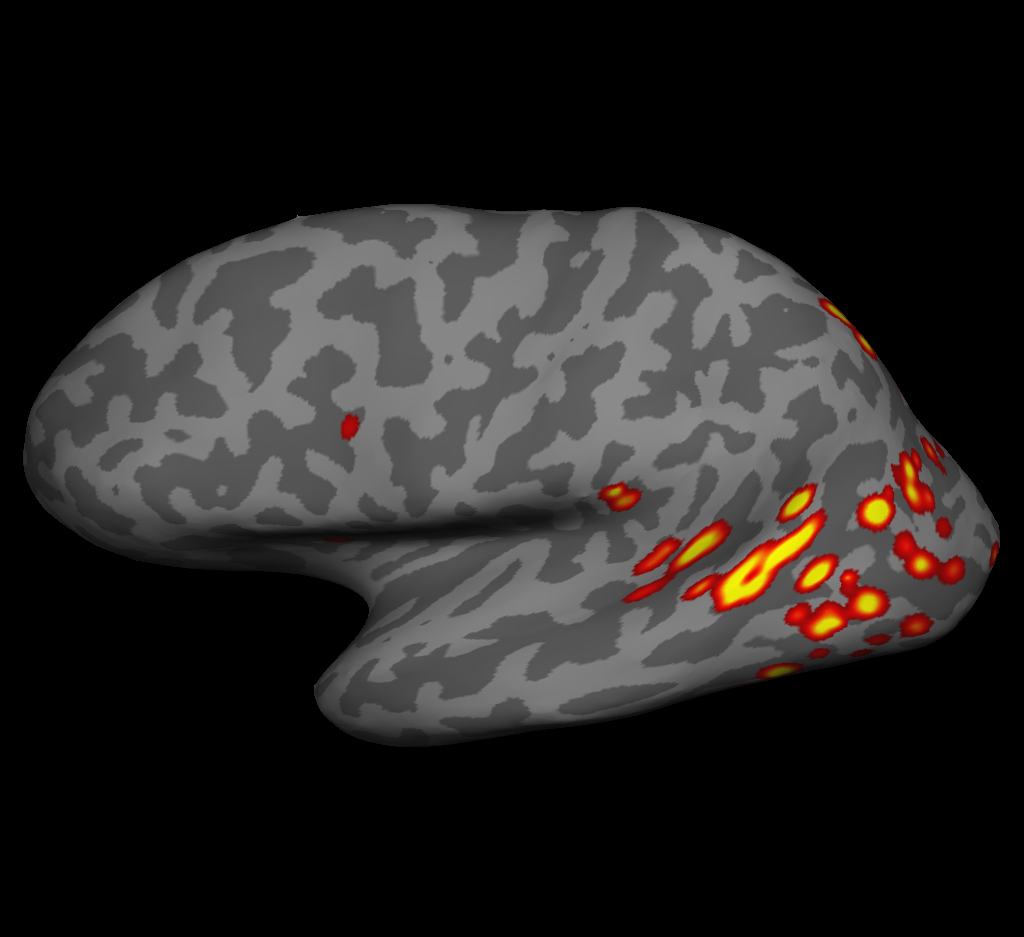
\includegraphics[width=\textwidth]{figures/s1-lh-lateral-sensitivity}
\caption{}
\end{subfigure}
\begin{subfigure}{0.4\textwidth}
\centering
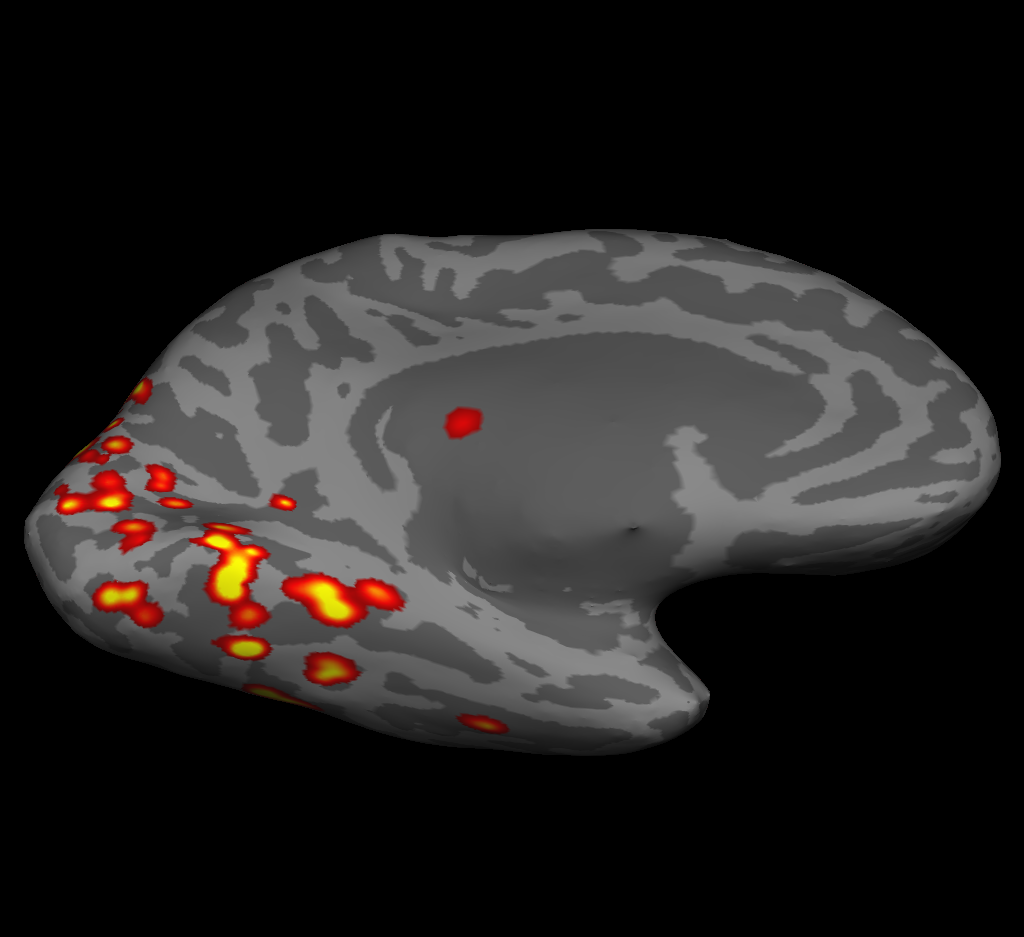
\includegraphics[width=\textwidth]{figures/s1-lh-medial-sensitivity}
\caption{}
\end{subfigure}
\begin{subfigure}{0.4\textwidth}
\centering
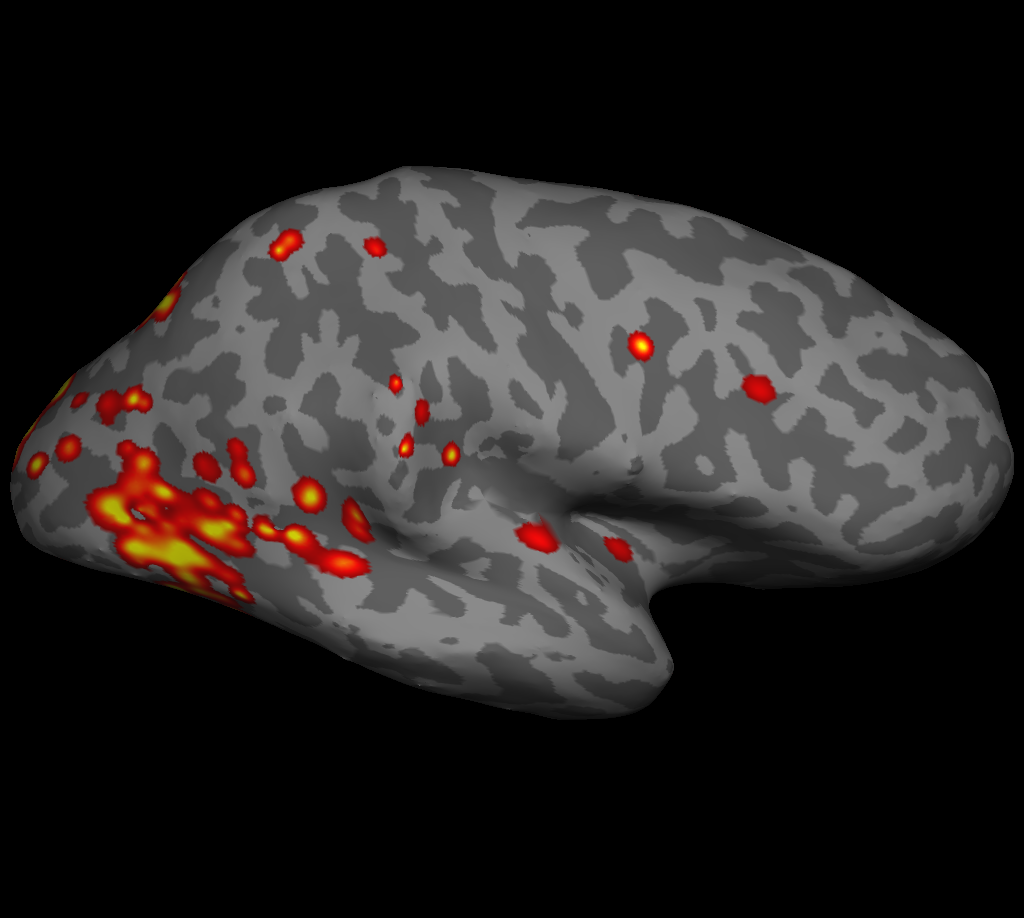
\includegraphics[width=\textwidth]{figures/s2-rh-lateral-sensitivity}
\caption{}
\end{subfigure}
\begin{subfigure}{0.4\textwidth}
\centering
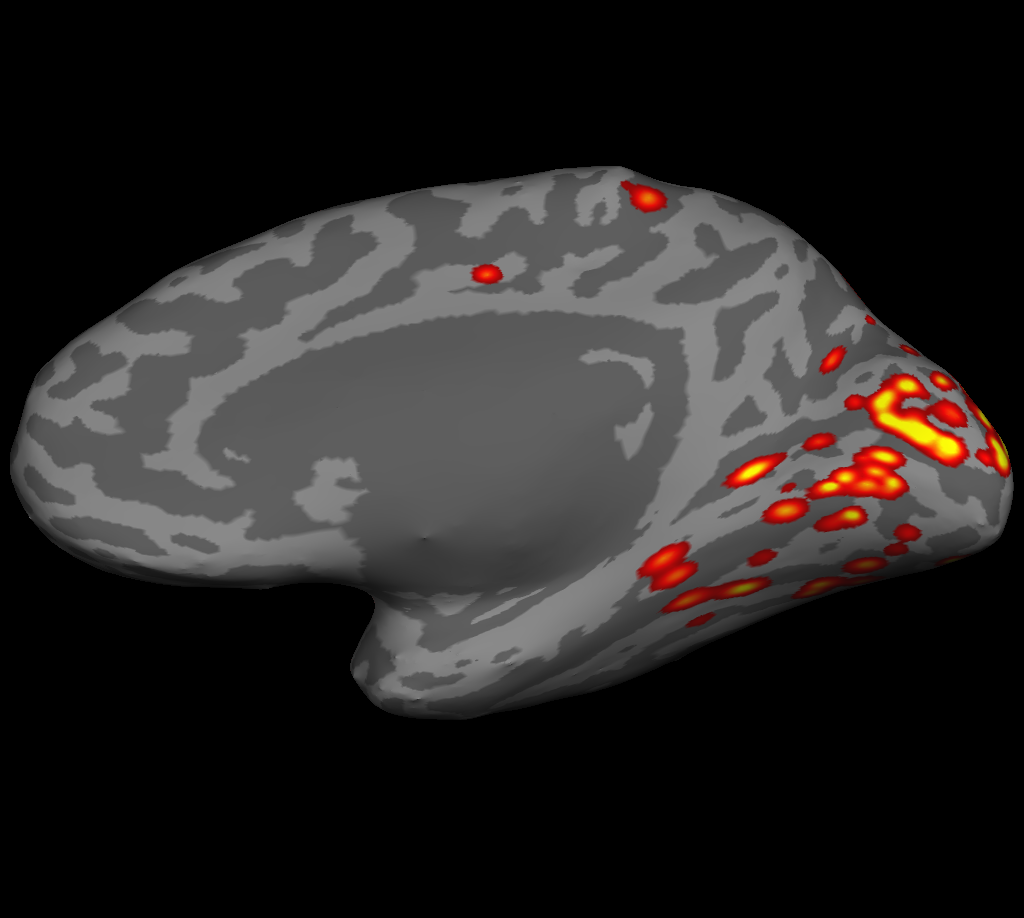
\includegraphics[width=\textwidth]{figures/s2-rh-medial-sensitivity}
\caption{}
\end{subfigure}
\begin{subfigure}{0.4\textwidth}
\centering
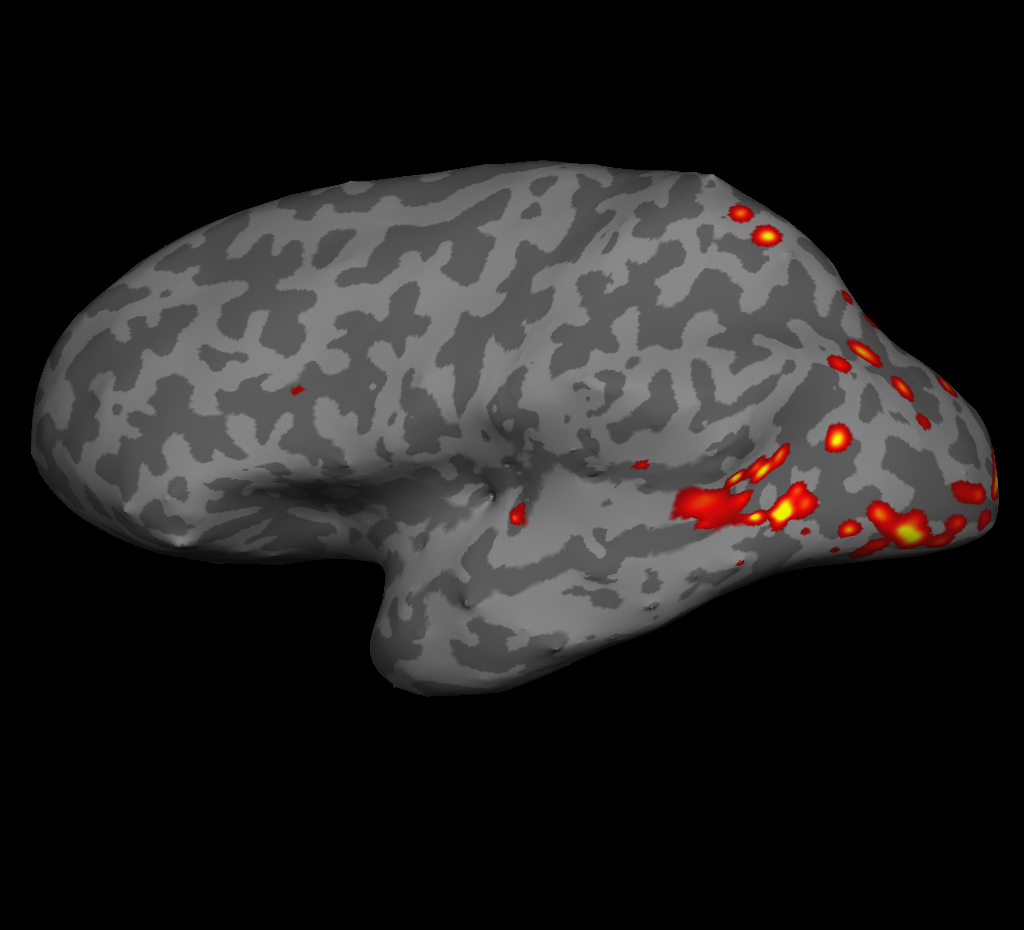
\includegraphics[width=\textwidth]{figures/s3-lh-lateral-sensitivity}
\caption{}
\end{subfigure}
\begin{subfigure}{0.4\textwidth}
\centering
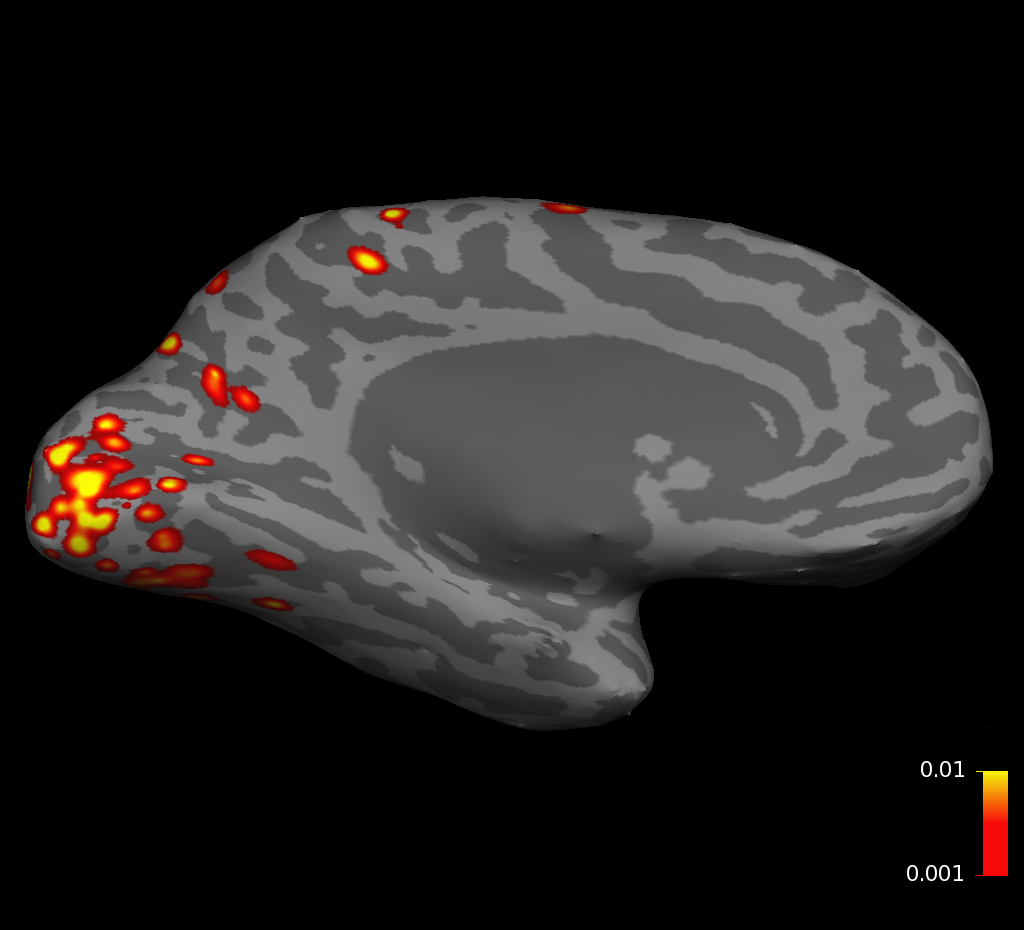
\includegraphics[width=\textwidth]{figures/s3-lh-medial-sensitivity}
\caption{}
\end{subfigure}
\caption{Individual sensitivity maps for three different subjects. 
The left hemisphere is presented for the first and third subjects while the right hemisphere is presented for the second subject.}
\label{fig:individual-sensitivity}
\end{figure*}

To better explore the relationship between sensitivity and classifier performance we plotted the performance of the classifier when trained on only a subset of the input voxels as determined by a minimum sensitivity cut off.
Figure \ref{fig:sensitivity-cutoff} shows this plot on top of the histogram of sensitivity values.
Interestingly, the performance of the classifier is not significantly affected until a majority of the voxels have been removed.


\begin{figure}
\centering
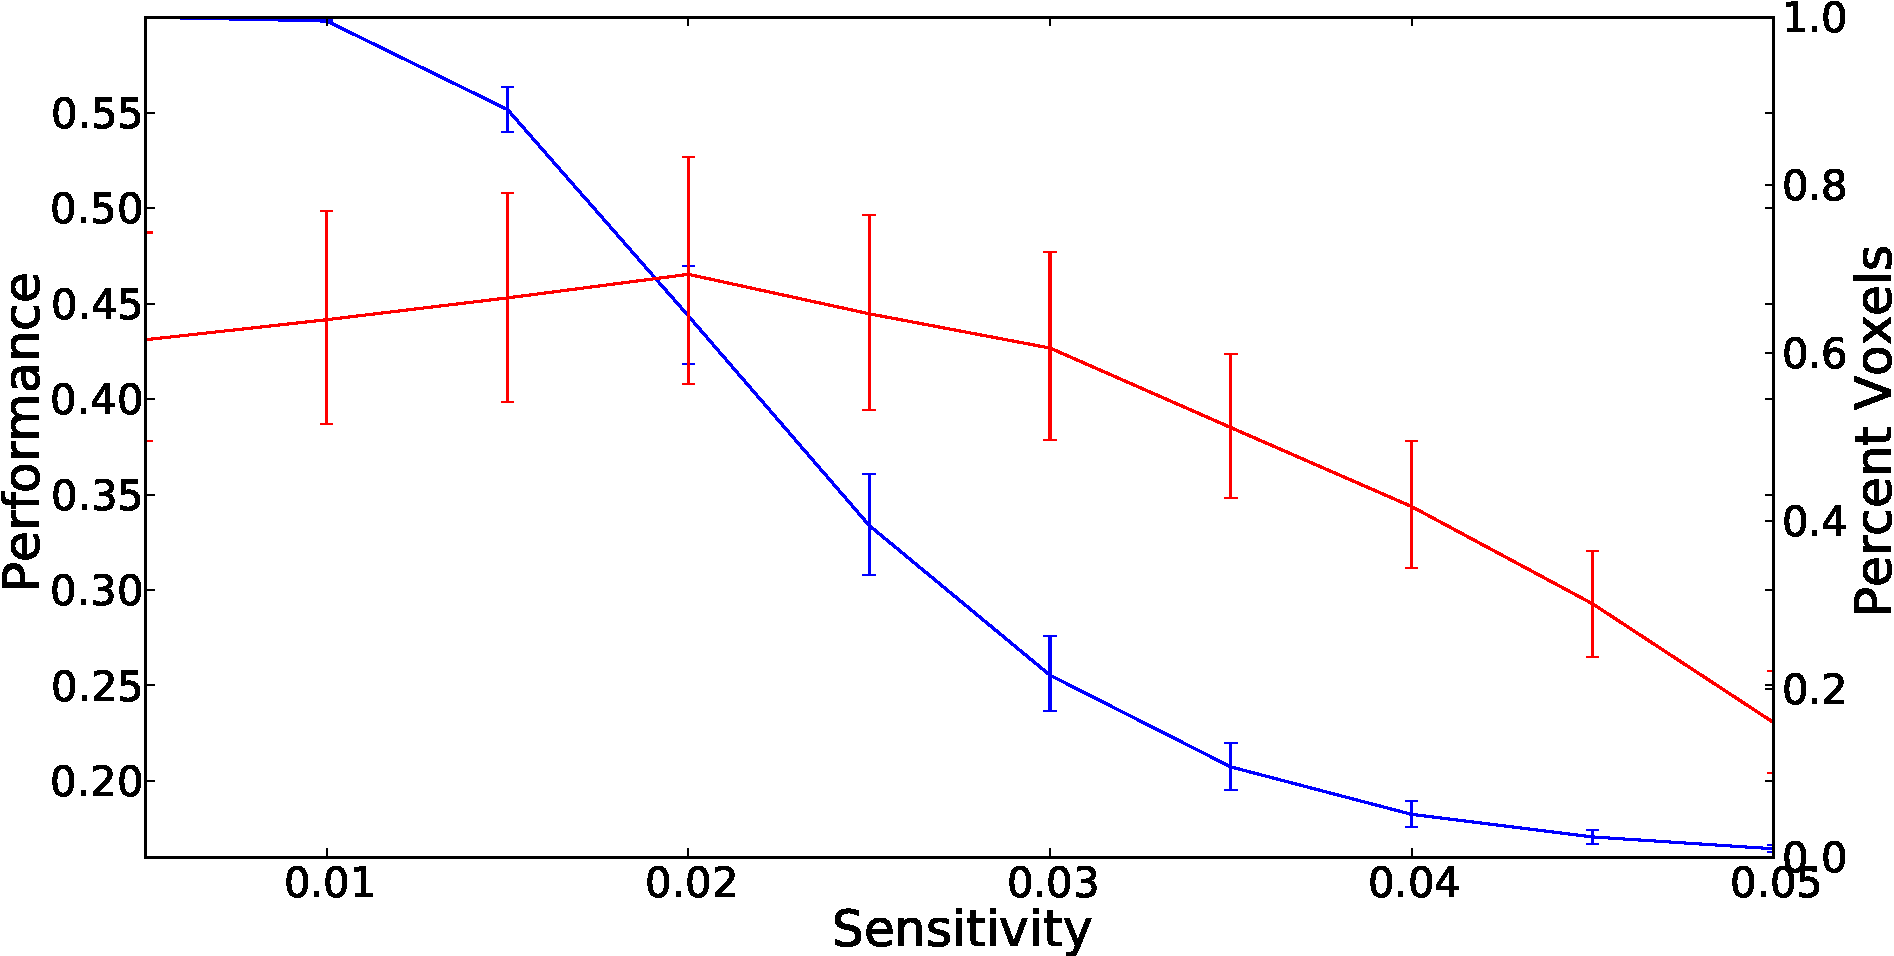
\includegraphics[width=0.4\textwidth]{figures/performance-verse-sensitivity-cutoff}
\caption{A histogram of the sensitivity analysis values and a plot of the feed forward neural network $F_1$ score when the inputs are pruned at a particular sensitivity value. }
\label{fig:sensitivity-cutoff}
\end{figure}

\section{Discussion}
Although both classifiers performed at well above chance levels for all subjects, the average performance on individual subjects varied significantly.
These variations could be the result of differences in age, general cognitive state, or simply how much attention the subject was paying to the stimulus during the scan.
The lack of a task during our stimulus makes these variations difficult to interpret since attention and cognitive state are not well controlled.
In future experiments, we plan to introduce a difficult task for the subjects to perform and we expect to see the average performance increase and the variation between subjects decrease.
However, the fact that the classifiers could still perform at well above chance levels without a focused task increases our confidence in the generalizability of the results of machine learning classifiers applied to fMRI data.


This could be a result of 6 characters being too much for the subject to consider individually.
Interestingly, the confusion is not often between 5 and 6 characters, but rather between 1 or 2 and 6 characters.
This would seem to indicate that when the number of characters grows too large, they are interpreted as a single unit.

The reported results are well above chance, indicating there is useful information about character number in the BOLD signal.
The sensitivity analysis indicates that no single region of the brain is responsible for counting characters, and there is not a simple linear relationship between magnitude of activation and cardinality.
Rather, it is a complex pattern of distributed activation requiring machine learning methods to capture the stimulus-response relationship.

Only a relatively small number of brain voxels were actually needed to perform the classifications with maximal performance. This could indicate that only a small number of voxels are relevant for classification, or that the information is highly redundant between voxels, or, most likely, some a combination of these two.
Specifically, the harmonic analysis will select some voxels that covary with the stimulus, but their patterns of activation may not be highly discriminative with respect to character count.
These voxels will also be assigned low sensitivity values by the trained classifiers.
On the other hand, brain responses themselves can show strong spatial correlations on the centimeter scale, particularly in the higher-order visual areas that dominate our sensitivity results. Voxels sampling these regions could all show similar classification sensitivity, but yield redundant information.
Therefore, high sensitivity is sufficient but not necessary for the localization of a function in a particular region.


Earlier, we presented this new trend in brain state classification as a departure from traditional fMRI experiments which seek to identify the purpose or function of particular brain regions. \emph{This was not clearly stated in the Intro!}
However, it is important to note that through sensitivity analysis these machine learning classifiers can be re-purposed for just that goal.
If a region of the brain is highly important for accurately predicting the presence of a particular stimulus then it logically follows that that region must somehow be involved in the processing of that stimulus.
Furthermore, multi-voxel non-linear machine learning classifiers can potentially identify much more complex interactions between brain regions than the simple GLM.

\bibliography{bib}

\end{document}
